\chapter{Forza magnatica e Campo magnetico}

I capitoli precedenti sono stati dedicati all'elettrostatica, ovvero allo studio delle interazioni tra cariche \emph{fisse}. Adesso però andremo a trattare dell'interazione delle cariche in moto, studio che è il fondamento della magnetostatica \mkeyword{magnetostatica}. \\

La proprietà di attirare la limatura di ferro, mostrata da alcuni minerali e in particolare dalla magnetite, era già nota nel VII secolo a.C., tuttavia la prima relazione tra fenomeni magnetici ed elettrici fu scoperta da Oersted nel 19° secolo e successivamente l'argomento fu approfondito soprattutto da Ampère. \\

Oersted mostrò che un ago magnetico, posto in prossimità di un filo percorso da corrente, tende ad assumere una ben definita posizione di equilibrio.\\
Se poniamo in un piano perpendicolare al filo percorso da corrente della limatura di ferro osserviamo che questa di addensa lungo circonferenze con centro il filo stesso. \\
Alla luce di quanto visto finora il risultato si interpreta dicendo che il filo percorso da corrente produce un \emph{campo magnetico} \mkeyword{campo magnetico}, che indichiamo con il simbolo $\mathbf{B}$.\\
In seguito Ampère dimostrò che anche due fili percorsi da corrente interagiscono e intuì che \emph{le azioni magnetiche non sono altro che la manifestazione dell'interazione tra cariche elettriche in movimento}.\\

Negli anni successivi Faraday dimostrò che l'esistenza di un'ulteriore connessione tra elettricità e magnetismo, provando che campi magnetici variabili nel tempo producono campi elettrici. Infine Maxwell dimostrò che nel caso più generale un \emph{campo elettrico e un campo magnetico non possono avere esistenza indipendente e vanno unificati nell'unico concetto di campo elettromagnetico}. 


\section{Legge di Gauss per il campo magnetico}

Le osservazioni sperimentali mettono in evidenza che il campo magnetico è una grandezza vettoriale e, in analogia a quanto fatto per il campo elettrostatico, è possibile dare una descrizione del campo magnetico in termini di linee di campo magnetico, \mkeyword{linee di campo magnetico} cioè quelle linee che sono in ogni punto tangenti al campo magnetico $\mathbf{B}$. \\

Per il campo magnetico $\mathbf{B}$, come per il campo elettrostatico $\mathbf{E}$, valgono le seguenti proprietà:

\begin{enumerate}
    \item una linea di campo magnetico è in ogni punto tangente e concorde al campo $\mathbf{B}$ in quel punto
    \item le linee del campo magnetico non si incrociano mai, in quanto in ogni punto il campo $\mathbf{B}$ è definito univocamente 
\end{enumerate}

Come detto sopra le azioni magnetiche non sono altro che la manifestazione dell'interazione tra cariche elettriche in movimento, quindi per descrivere le azioni sui magneti bisogna pensare che in ogni atomo o in ogni molecola devono esistere delle correnti microscopiche locali, che prendono il nome di \mkeyword{correnti amperiane}correnti molecolari di Ampère o correnti amperiane. Ampère provò l'equivalenza tra un circuito percorso da corrente e un dipolo magnetico, sia rispetto alle forze subite ad opera di un campo magnetico, sia per quanto riguarda il campo magnetico prodotto. Avendo allora già sviluppato il formalismo relativo ai dipoli elettrici, è comodo utilizzarlo anche per le azioni magnetiche, senza dargli però un significato fisico profondo.\\

Consideriamo adesso una superficie chiusa $\Sigma$ che racchiuda nel suo interno un magnete permanente o una parte di esso 

\begin{figure} [h]
    \centering
    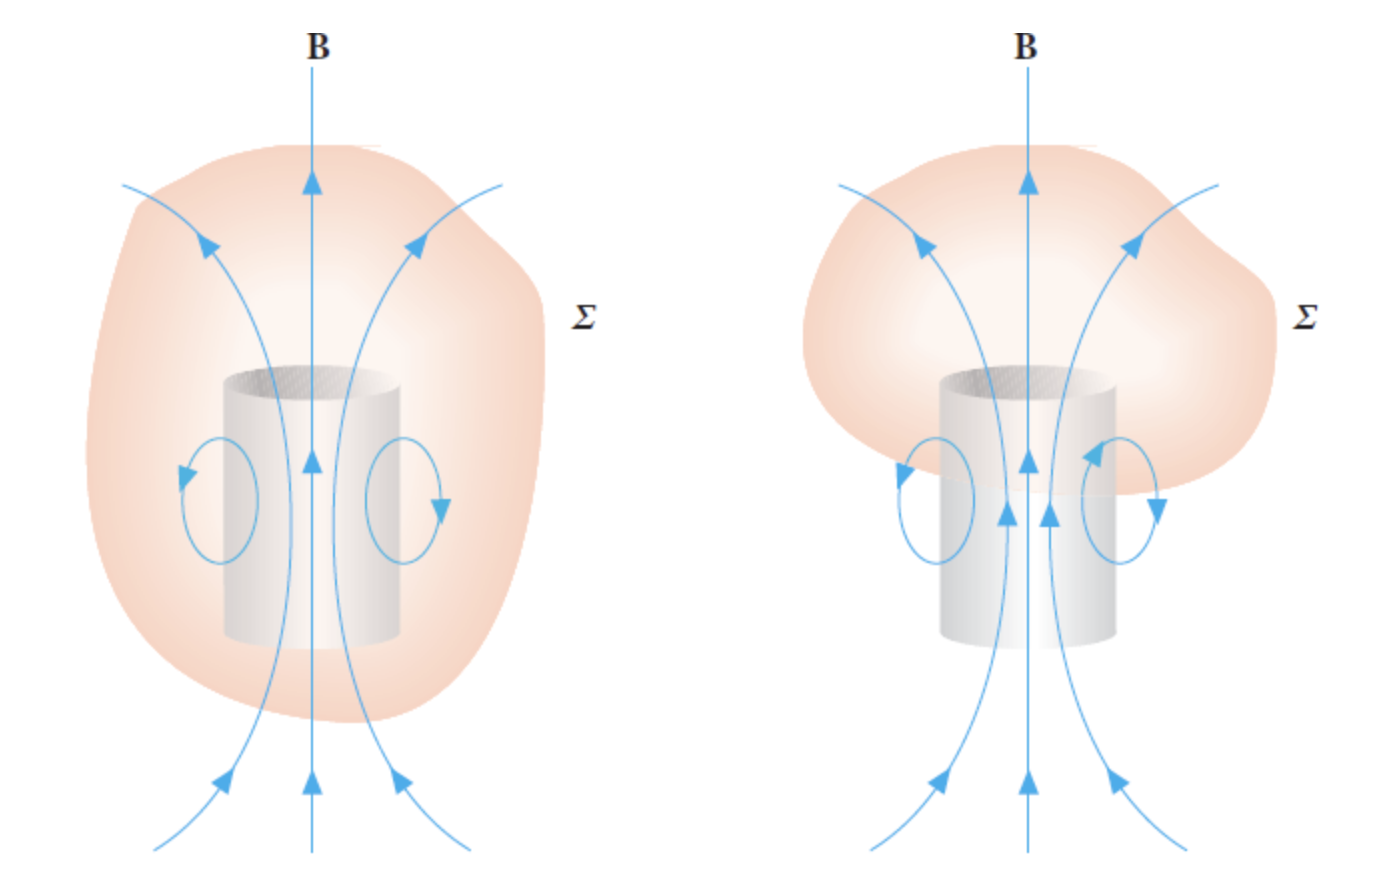
\includegraphics[width=0.75\linewidth]{figure/image40.png}
    \caption{Superficie chiusa che racchiude un magnete permanente}
    \label{fig:chapter_13_1}
\end{figure}


L'equivalenza formale tra le correnti microscopiche e i dipoli magnetici comporta che in entrambi i casi nell'interno della superficie $\Sigma$ sia contenuto un numero intero di dipoli magnetici: una superficie infatti non può mai tagliare uno di questi ipotetici dipoli elementari, operazione che, se i dipoli esistessero realmente, equivarrebbe a isolare due monopòli magnetici Sud e Nord. \\

Da questo punto di vista, la struttura dipolare comporta che la somma delle ipotetiche masse magnetiche sia nulla, per cui per il campo magnetico si può enunciare la legge di Gauss \mkeyword{Legge di Gauss per il campo magnetico}

\begin{tcolorbox}[colback=yellow!10!white, colframe=orange!70!black, boxrule=0.8pt]
\begin{equation}
    \Phi (\mathbf{B}) = \oint_{\Sigma} \mathbf{B} \cdot \mathbf{u}_n \ d \Sigma = 0
\end{equation}
\end{tcolorbox}

Il flusso del campo magnetico attraverso una qualunque superficie chiusa $\Sigma$ è sempre nullo. \\

In termini locali 

\begin{tcolorbox}[colback=yellow!10!white, colframe=orange!70!black, boxrule=0.8pt]
\begin{equation}
    \nabla \cdot \mathbf{B} = 0
\end{equation}
\end{tcolorbox}

Di conseguenza il flusso di $\mathbf{B}$ attraverso le superfici che hanno lo stesso contorno e sono concordemente orientate è sempre lo stesso e si può così parlare in maniera univoca di flusso del campo magnetico attraverso una linea chiusa, ovvero il flusso concatenato con una linea chiusa. \mkeyword{flusso concatenato}

\section{Forza magnetica su una carica in moto}

Consideriamo una particella di massa $m$ e carica $q$, posta in un campo magnetico $\mathbf{B}$. \\

Se la particella è ferma in un sistema di riferimento solidale alle sorgenti del campo magnetico si trova che su di essa non agisce nessuna forza, in accordo con il fatto che l'interazione magnetica si manifesta solamente tra cariche in movimento. \\

Se invece la particella è in moto con velocità $\mathbf{v}$ rispetto al sistema di riferimento suddetto, si verifica che su di essa agisce la \emph{forza di Lorentz} \mkeyword{forza di Lorentz}

\begin{tcolorbox}[colback=yellow!10!white, colframe=orange!70!black, boxrule=0.8pt]
\begin{equation}
    \mathbf{F} = q \mathbf{v} \times \mathbf{B}
\end{equation}
\end{tcolorbox}

Una particolarità di questa forza è il fatto che essa è sempre ortogonale alla velocità, cioè alla traiettoria, e pertanto in base alla definizione di lavoro si ha 

\begin{equation}
    d W = \mathbf{F} \cdot d \mathbf{s} = q \ (\mathbf{v} \times \mathbf{B}) \cdot \mathbf{v} \ dt = 0
\end{equation}

In quanto il vettore $(\mathbf{v} \times \mathbf{B})$ è perpendicolare a $\mathbf{v}$. Pertanto risulta che \emph{la forza di Lorentz non compie lavoro sulla particella}. \\

Questo comporta che l'energia cinetica rimane costante e quindi \emph{quando una particella carica si muove in un campo magnetico la sua velocità cambia in direzione, ma non in modulo}. 

\subsection{Moto in campo magnetico uniforme, $\mathbf{\theta = \pi/2}$}

Supponiamo che il campo magnetico $\mathbf{B}$ sia uniforme in una certa regione e che la velocità iniziale della particella sia ortogonale a $\mathbf{B}$: la forza di Lorentz, anch'essa ortogonale a B, produce una variazione della direzione della velocità ancora ortogonale a B e quindi la velocità in qualsiasi istante successivo sta nel piano ortogonale a B individuato dalla velocità iniziale. \\

\begin{figure}[h]
    \centering
    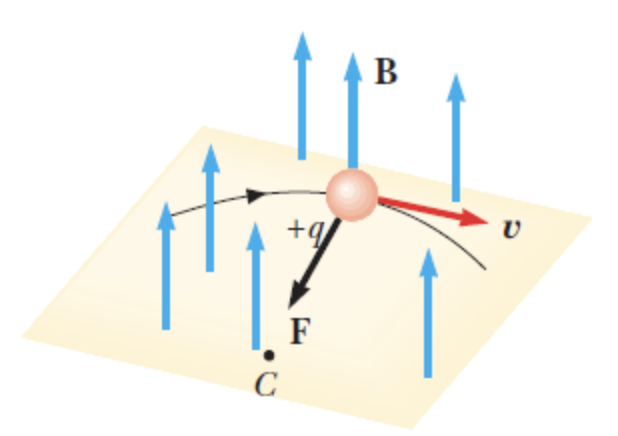
\includegraphics[width=0.37\linewidth]{figure/image41.png}
    \caption{Moto di una carica in un campo magnetico uniforme perpendicolare alla velocità}
    \label{fig:chapter_13_2}
\end{figure}

La legge del moto è

\begin{equation}
    F = q v B = m a_n = m \frac{v^2}{r}
\end{equation}

Pertanto il moto è \emph{circolare uniforme} e il raggio di curvatura $r$ risulta essere

\begin{tcolorbox}[colback=yellow!10!white, colframe=orange!70!black, boxrule=0.8pt]
\begin{equation}
    r = \frac{mv}{qB} = \frac{p}{qB}
\end{equation}
\end{tcolorbox}

Inoltre si ricava facilmente che 

\begin{tcolorbox}[colback=yellow!10!white, colframe=orange!70!black, boxrule=0.8pt]
\begin{equation}
    \omega = \frac{v}{r} = \frac{qB}{m} \quad ; \quad T = \frac{2 \pi}{\omega} = \frac{2 \pi m}{qB}
\end{equation}
\end{tcolorbox}

\subsection{Moto in campo magnetico uniforme, $\theta$ generico}

Se l'angolo $\theta$ che la velocità della particella forma con il campo magnetico è qualsiasi, scomponiamo la velocità $\mathbf{v}$ nelle due componenti $v_n = v \sin \theta$ ortogonale a $\mathbf{B}$ e $v_p = v \cos \theta $ parallela a $\mathbf{B}$. 

\begin{figure} [h]
    \centering
    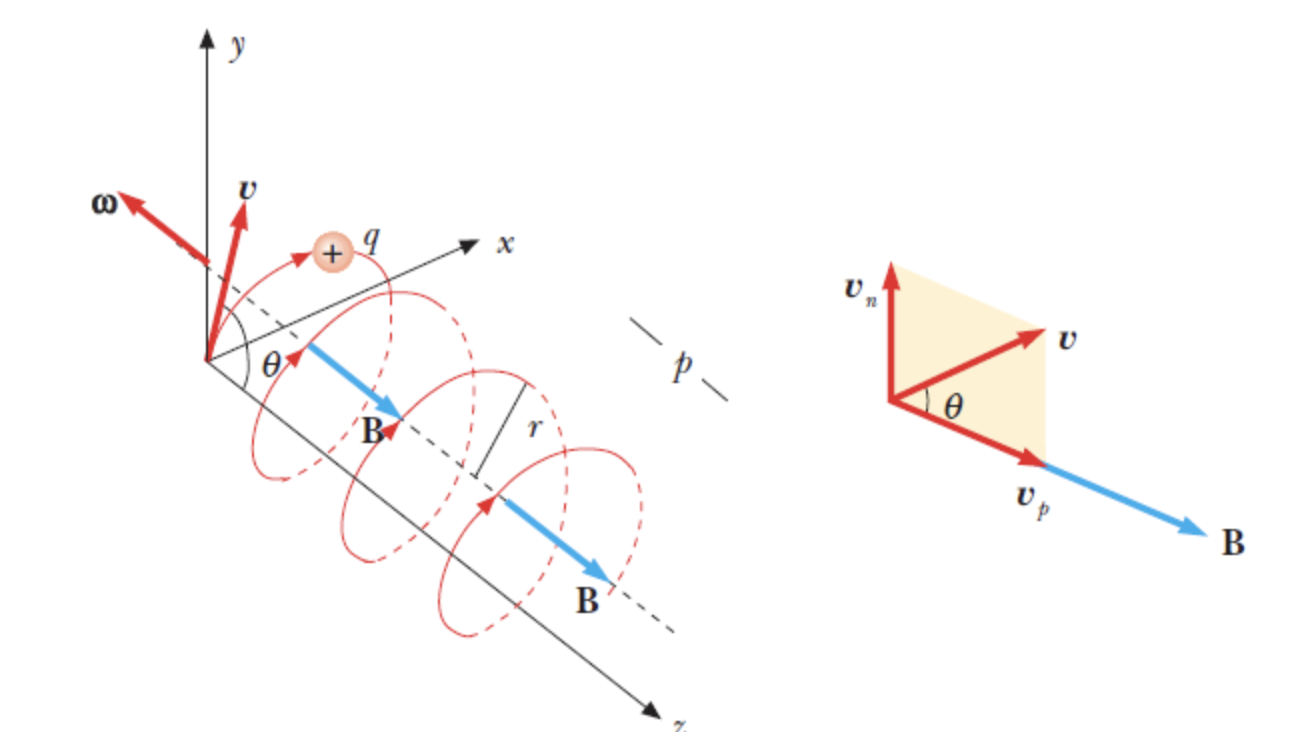
\includegraphics[width=0.7\linewidth]{figure/image42.png}
    \caption{Moto elicoidale di una particella con carica positiva in campo magnetico uniforme}
    \label{fig:chapter_13_3}
\end{figure}

La forza magnetica che agisce sulla particella è

\begin{equation}
    \mathbf{F} = q \mathbf{v}_n \times \mathbf{B} 
\end{equation}

Abbiamo pertanto in un piano ortogonale a $\mathbf{B}$ un moto circolare uniforme con velocità $v_n$, eguale a quello descritto nel caso precedente; svolgendo gli stessi ragionamenti precedenti, si ottiene

\begin{tcolorbox}[colback=yellow!10!white, colframe=orange!70!black, boxrule=0.8pt]
\begin{equation}
    r = \frac{mv \sin \theta}{q B}
\end{equation}
\end{tcolorbox}

\newpage

\section{Forza magnetica su un conduttore percorso da corrente}

La corrente elettrica in un conduttore è dovuta al moto degli elettroni sotto l'azione del campo elettrico applicato tramite un generatore, pertanto quando il conduttore percorso da corrente è immerso in un campo magnetico a ciascun elettrone è applicata la forza di Lorentz:

\begin{equation*}
    \mathbf{F}_L = - e \mathbf{v}_d \times \mathbf{B}
\end{equation*}

Quindi in un tratto lungo $d s$ e si sezione $\Sigma$ sono contenuti $n \Sigma \ ds$ elettroni e la forza risultante è 

\begin{equation*}
    d \mathbf{F} = n \Sigma \ ds \ \mathbf{F}_L = - (\Sigma ds) n e \mathbf{v}_d \times \mathbf{B} = \Sigma ds \ \mathbf{j} \times \mathbf{B}
\end{equation*}

Essendo $\Sigma ds$ eguale al volume infinitesimo $d\tau$, si vede che la forza agente per unità di volume sul conduttore è

\begin{tcolorbox}[colback=yellow!10!white, colframe=orange!70!black, boxrule=0.8pt]
\begin{equation}
    \mathbf{F}_{\tau} = \mathbf{j} \times \mathbf{B}
\end{equation}
\end{tcolorbox}

D'altra parte, \emph{riferendoci a un conduttore filiforme} e ricordando che $\Sigma j$ è la corrente $i$ che percorre il filo, oritentiamo $d \mathbf{s}$ come $\mathbf{j}$ e otteniamo 

\begin{tcolorbox}[colback=yellow!10!white, colframe=orange!70!black, boxrule=0.8pt]
\begin{equation} \label{eq:seconda_legge_elementare_Laplace}
    d \mathbf{F} = i \ d \mathbf{s} \times \mathbf{B}
\end{equation}
\end{tcolorbox}

Questa relazione è nota come seconda legge elementare di Laplace. \mkeyword{seconda legge fondamentale di Laplace}\\

Allora per ottenere la forza su un tratto di filo indeformabile di lunghezza infinita, percorsa da corrente (stazionaria) $i$, si integra la \ref{eq:seconda_legge_elementare_Laplace}:

\begin{tcolorbox}[colback=yellow!10!white, colframe=orange!70!black, boxrule=0.8pt]
\begin{equation} \label{eq:seconda_legge_elementare_Laplace_integrata}
    \mathbf{F} = i \int_{P}^{Q}\ d \mathbf{s} \times \mathbf{B}
\end{equation}
\end{tcolorbox}

Dove $P$ e $Q$ sono gli estremi del filo. \\

\subsection{Campo magnetico uniforme e filo rettilineo}

Supponiamo che il campo magnetico sia uniforme e che il conduttore sia rettilineo, di lunghezza l. Allora la \ref{eq:seconda_legge_elementare_Laplace_integrata} si semplifica in

\begin{equation*}
    \mathbf{F} = i \left( \int_{P}^{Q} d \mathbf{s} \right) \times \mathbf{B}
\end{equation*}

in quanto sia il modulo del campo che l'angolo $\theta$ formato con $d \mathbf{s}$ sono costanti durante l'integrazione, e si ha 

\begin{tcolorbox}[colback=yellow!10!white, colframe=orange!70!black, boxrule=0.8pt]
\begin{equation} 
     \mathbf{F} = i \mathbf{l} \times \mathbf{B}
\end{equation}
\end{tcolorbox}

\subsection{ Campo magnetico uniforme e filo curvilineo piano}

Supponiamo ora che il campo magnetico sia uniforme, ma che il filo non sia rettilineo: esso può essere anche curvilineo, purché giaccia interamente in un piano (ad esempio il piano $xy$). \\

\'E facile verificare che 

\begin{tcolorbox}[colback=yellow!10!white, colframe=orange!70!black, boxrule=0.8pt]
\begin{equation} 
     \mathbf{F} = i \mathbf{PQ} \times \mathbf{B}
\end{equation}
\end{tcolorbox}

Pertanto la forza su un filo percorso da corrente che giace in un piano in cui agisce un campo magnetico uniforme $\mathbf{B}$ non dipende dalla forma del filo, ma solo dalla lunghezza del segmento che unisce i suoi estremi. \\

Inoltre \emph{la forza su un circuito che sta su un piano in cui agisce un campo magnetico $\mathbf{B}$ uniforme è nulla.}

